% -*- mode: fundamental -*-

% ****************************************************************

\chapter{BSV: Verifying BSV designs}

\markboth{Ch \arabic{chapter}: BSV: Verification}{\copyrightnotice}

\setcounter{page}{1}
% \renewcommand{\thepage}{\arabic{page}}
\renewcommand{\thepage}{\arabic{chapter}-\arabic{page}}

\label{ch_BSV_verification}

% ****************************************************************

\section{Introduction}

In this chapter we describe general techniques used to verify BSV
designs of any kind.  The next chapter focuses on techniques for
verification of CPU implementations.

% ****************************************************************

\section{BSV: Testbenches and DUTs}

\index{BSV!Testbench}
\index{BSV!DUT}

To debug a BSV design, we typically set up a system similar to that
shown in Figure~\ref{Fig_Testbench_DUT}.
\begin{figure}[htbp]
  \centerline{\includegraphics[width=6in,angle=0]{Figures/Fig_Testbench_DUT}}
  \caption{\label{Fig_Testbench_DUT}
           A testbench connected to a DUT}
\end{figure}
The BSV design that is being tested is usually called the ``Design
Under Test'', or DUT for short.  The surrounding and/or adjacent
modules are called the ``Testbench'' (or ``Test Harness'' or ``Test
Environment'').

The top-level module, \verb|mkTop|, has the \verb|Empty| interface,
which is just an interface with no methods, and is pre-defined in the
\emph{bsc} library.

The testbench interacts with the DUT {\via} its interface methods.
The DUT interface and the testbench interface are often opposite
``duals'', {\eg} if \verb|DUT_IFC| has \verb|FIFOF_I| sub-interface
for input data, the testbench might have a corresponding
\verb|FIFOF_O| that delivers that input data; these are connected
together by \verb|mkTop|.

Code inside the testbench produces input data for the DUT; this part
of the testbench is called the ``stimulus generator''.  Stimulus data
can be generated in the testbench, or read from data files.

Other code inside the testbench collects output data from the DUT and
checks if it has the expected value corresponding to the stimulus.
This part of the testbench is called a ``checker''.  Output data can
be checked immediately in the testbench, or recorded into files for
offline manual or automated checking.  Alternatively, the DUT may just
print outputs to the screen (during simulation), which can be visually
examined for correctness or recorded for offline manual or automated
checking.

BSV designers typically write their testbenches in BSV.  If the
testbench is only used in simulation (not in actual hardware, FPGA or
ASIC) then it can read and write files.  It can also import C code
(see Appendix~\ref{Sec_Importing_C}) to reuse existing C algorithms
and models, and to have full access to operating system services
(files, networking, {\etc}).

In the SystemVerilog community there is a mature standard methodology
for testbenches called UVM (Unversal Verification Methodology) which
exploits the ``object-orientd programming'' aspects of SystemVerilog
for reusability (see Glossary~\ref{apx_Glossary} for some more
detail).  BSV designs can also use UVM testbenches.  The whole of
Figure~\ref{Fig_Testbench_DUT} can be in Verilog/SystemVerilog, with
the DUT using the Verilog produced from a BSV design using the
\emph{bsc} compiler.

% ****************************************************************

\section{BSV: ``{\tt printf}''-style Debugging}

\index{BSV!printf@{\tt printf}-style debugging}

A popular style of debugging BSV designs is the same as in debugging
software in any programming language: insert ``print'' statements in
the BSV code at various places to print out values of interest during
simulation.  We examine these outputs to identify suspicious values
and then perhaps insert and remove print statements to zero-in on the
exact place in the BSV code where something wrong was computed.

BSV, like Verilog and SystemVerilog, has the following built-in
functions to write to files during simulation, analogous to ``{\tt
printf}'' in C. All of them have {\tt Action} type, and so they can
occur in any Action context: bodies of rules, bodies of Action and
ActionValue methods, bodies of Action and ActionValue functions.

{\tt
\begin{tabbing}
\hmmm\= \$fdisplay \= ( {\it file}, \= {\it format-string}, {\it arg}, ..., {\it arg} ) \kill
     \> \$write    \> (             \> {\it format-string}, {\it arg}, ..., {\it arg} ) \\
     \> \$display  \> (             \> {\it format-string}, {\it arg}, ..., {\it arg} ) \\
\\
     \> \$fwrite   \> ( {\it file}, \> {\it format-string}, {\it arg}, ..., {\it arg} ) \\
     \> \$fdisplay \> ( {\it file}, \= {\it format-string}, {\it arg}, ..., {\it arg} )
\end{tabbing}
}

The first two write to ``standard output'' ({\ie} the terminal), and
the latter two write to a specific file which has previously been
opened with an Action statement like this:

{\tt
\begin{tabbing}
\hmmm {\it file} <- \$fopen ("log.txt", "w");
\end{tabbing}
}

The difference between ``write'' and ``display'' is merely that the
latter appends a newline at the end of the output.

These are similar to C's \verb|printf| and \verb|fprintf| functions.
The format string is a string (in double-quotes) with formatting
directives for the arguments that follow (\verb|%d| for signed
integers, \verb|%b| for binary numbers, \verb|%h| for hexadecimal
numbers, {\etc}).

These BSV statements for printing only exist in simulation code.  They
are omitted completely by synthesis tools that target actual hardware
(ASIC or FPGA).\footnote{This is not because of any fundamental
synthesizability difficulty, it is only because there is no standard
concept of ``file'' or ``output stream'' in hardware designs, not even
a serial port.}

% ================================================================

\subsection{{\tt FShow} for ``pretty-printing'' enums and structs}

\index{BSV!FShow@{\tt FShow}!Standard Typeclass containing the {\tt fshow()} function}
\index{BSV!fshow@{\tt fshow}!Standard overloaded function producing {\tt Fmt}
objects for various types}

In any enum or struct type declaration in BSV, one can attach a
``\verb|deriving(FShow)|'' clause to request the \emph{bsc} compiler
to define an ``\verb|fshow|'' function for the type, with some default
formatting.  For example, the Drum/Fife code has such a clause in the
declaration of the \verb|Decode_to_RR| struct type:

\input{Code_Extracts/Decode_to_RR.tex}

The result-type of \verb|fshow()| is of type ``\verb|Fmt|'', and this
type is also allowed as an argument to \verb|$display| (and its
variants):  Example:

{\small
\begin{Verbatim}[frame=single, numbers=left]
   Decode_to_RR y = ...
   Fmt          f = fshow (y);
   $display (      "Decode result is ", f);
   $fwrite  (file, "Decode result is ", f);
\end{Verbatim}
}

% ================================================================

\subsection{{\tt Fmt} formatted values}

\index{BSV!Fmt@{\tt Fmt}!formatted object}
\index{BSV!Formatted output using {\tt Fmt} objects}

BSV's formatting facilities are actually more powerful than
\verb|printf| in C/C++ or \verb|$display| in Verilog/SystemVerilog.

The result-type of \verb|fshow()| is a standard type in BSV called
\verb|Fmt|, and this is also an acceptable argument in BSV's
\verb|$display| functions (as demonstrated above in the last section).

We can create new \verb|Fmt| objects using the built-in pure function
\verb|$format()|, and we can combine them (concatenate them) using an
infix ``\verb|+|'' operator.  \verb|Fmt| is a first-class type, so we
can bind it to variables, pass it as arguments and results of
functions, and so on.  The following example illustrates defining
another function to format a \verb|Decode_to_RR| struct type, an
alternative to \verb|fshow| to format it in some other preferred way:

\input{Code_Extracts/fshow_Decode_to_RR.tex}

Note the use of if-then-else to customize the \verb|Fmt| object
according to the actual data in the struct (which would not happen in
the default \verb|fshow()|, which would simply print all the struct
fields).  This function can be used just like, and in place of,
\verb|fshow|:

{\small
\begin{Verbatim}[frame=single, numbers=left]
   Decode_to_RR y = ...
   Fmt          f = fshow_Decode_to_RR (y);
   $display (      "Decode result is ", f);
   $fwrite  (file, "Decode result is ", f);
\end{Verbatim}
}

This shows one immediate advantage of the \verb|Fmt| facilities: we
can format something once and write it to multiple output streams.  By
abstracting formatting into a common function, it can be modified
easily and all \verb|$display| statements using it can share the
benefit.

A second advantage is that actual formatting code, which is often
quite verbose, \emph{ad hoc} and messy with a lot of fragments of
character strings, can be lifted to a different location in the code,
keeping the \verb|$display| statement short and sweet.

% ****************************************************************

\section{BSV: Dynamic assertions}

\index{BSV!assertions for debugging}

The BSV libraries offer a package:

{\tt
\begin{tabbing}
\hmmm import Assert :: *;
\end{tabbing}
}

which contains the following function:

{\tt
\begin{tabbing}
\hmmm function Action dynamicAssert(Bool b, String s);
\end{tabbing}
}

This can be used in any Action context ({\eg} a rule body) to check an
expected property each time that Action context is executed.  For
example the Drum CPU code includes the following excerpt:

{\small
\begin{Verbatim}[frame=single, numbers=left, label=src\_Drum/CPU.bsv]
   Action a_Retire_DMem =
   action
      ...
      let mem_rsp <- pop_o (to_FIFOF_O (f_DMem_rsp));
      dynamicAssert ((mem_rsp.rsp_type != MEM_REQ_DEFERRED),
                     "Mem req not speculative but got DEFERRED mem response");
      ...
   endaction
\end{Verbatim}
}

which checks for the unexpected situation where the DMem memory
response was ``deferred'' (deferred memory responses are only possible
for speculative memory accesses, which only occur in Fife and not in
Drum).  Every time this action is executed (on every DMem response),
the boolean condition is tested and, if false, it aborts the
simulation after printing the associated string.

These \verb|dynamicAssert| statements have no cost in final real
hardware because, like \verb|$display| statements, they exist only in
simulation code.  Thus, one should not hesitate to use them liberally.

% ****************************************************************

\section{BSV: Waveform-style debugging}

\index{BSV!VCD waveform dumping}
\index{BSV!Waveform dumping (VCDs)}
\index{BSV!Value Change Dump (VCD) waveform dumping}

Many hardware designers like to debug designs using ``waveforms'',
which are a graphical display of how values on buses (bundles of
wires) in the design vary over time.

All Verilog, SystemVerilog and VHDL simulators have a facility to
write out a ``Value Change Dump'' (VCD) file, which is a record of how
each bus (bundle of wires) in the design changed over time (measured
with clock ticks).  VCD files can then be viewed as a graphical
display in any waveform viewer.  Waveform viewers are bundled with
most commercial RTL simulators, but the free and open-source
\emph{gtkwave} viewer is also popular.

When simulating in a Verilog simulator, most simulators have
command-line or interactive controls to switch VCD dumping on or off.

When simulating in Bluesim interactively, the commands:

\begin{tabbing}
\hmmmm \= {\tt sim vcd on}  \hmm \= enables writing out VCDs \\
       \> {\tt sim vcd off}      \> disables  writing out VCDs
\end{tabbing}

VCD dumping can also be controlled from within a BSV program, using
these three Actions:

\begin{tabbing}
\hmmmm \= {\tt \$dumpvars} \hmm \= Starts writing out VCDs \\
       \> {\tt \$dumpoff}       \> Stops  writing out VCDs \\
       \> {\tt \$dumpon}        \> Resumes writing out VCDs
\end{tabbing}

% ****************************************************************
